\vspace{-0.05in}
\section{Range Expanding Migration Candidates}
\label{rangeexpansion}
\vspace{-0.05in}

In the prior section, we demonstrated that aggressively migrating pages generally improves application performance
by increasing the fraction of touches to a page serviced by higher-bandwidth (GPU-attached) GDDR versus (CPU-attached) DDR memory.  This
aggressive migration comes with high overheads in terms of TLB shootdowns and costly GPU pipeline stalls.  
One reason the legacy application directed {\tt memcpy} approach works well is that it performs both aggressive 
up-front data transfer to GDDR and does not require TLB shootdowns and stalls.  
Unfortunately, this requirement for application-directed transfer is not well suited to 
unified globally addressable memory with dynamic allocation-based programming models. 
In this section, we discuss a prefetching technique that can help regain the performance 
benefits of bulk memory copying between private memories, without the associated programming
restrictions.

Ideally, a page migration system prefetches pages into GDDR after they are allocated and populated in DDR, 
but before they are needed on the GPU\@.  Studying the results of the threshold-based migration experiments, 
we observe that pages often are migrated too late to have enough post-migration accesses to justify the 
cost of the migration.  One way to improve the timeliness of migrations is via a prefetching scheme 
we call \emph{range expansion}.   Range expansion builds on the baseline single-page migration mechanism
discussed previously. To implement basic range expansion, when the CUDA runtime is provided a virtual address to
be migrated, the runtime also schedules an additional \emph{N} pages in its (virtual address) neighborhood 
for migration.  Pages are inserted into the migration queue in the order of furthest, from the triggered address,
to the nearest, to provide the maximum prefetching affect based on spatial locality.
We then vary this range expansion amount \emph{N} from 0--128 and discuss the results in Section~\ref{rangeexpansionresults}.

The motivation for migrating (virtually) contiguous pages can be seen in
Figure~\ref{fig:cdfannotation}. The figure shows virtual page addresses that are
touched by the GPU for three applications in our benchmark set.
The X-axis shows the fraction of the application footprint when
sampled, after on-chip caches, at 4KB page granularity and sorted from
{\color{black}most to fewest accesses.
The primary Y-axis (shown figure left) shows the cumulative distribution
function of memory bandwidth among the pages allocated by the application.
Each point on the secondary scatter
plot (shown figure right) shows the virtual address of the corresponding page on
the x-axis. This data reveals that hot and cold pages are strongly clustered within the
virtual address space.  However, the physical addresses of these pages will be
non-contiguous due to address interleaving performed by the memory controller.
} This clustering
is key to range expansion because it suggests that if a page is identified for migration, then other 
neighboring pages in the virtual address space are likely to have a similar number of total touches.  
To exploit this property,
range expansion migrates neighboring virtual addresses of a migration candidate \emph{even if they
have not yet been accessed on the GPU}\@.  By migrating these pages before they are touched on the GPU, range
expansion effectively prefetches pages to the higher bandwidth memory on the GPU, 
improving the timeliness and effectiveness of page migrations.  

\begin{figure}[pth]
    \centering
    \subfloat[bfs]{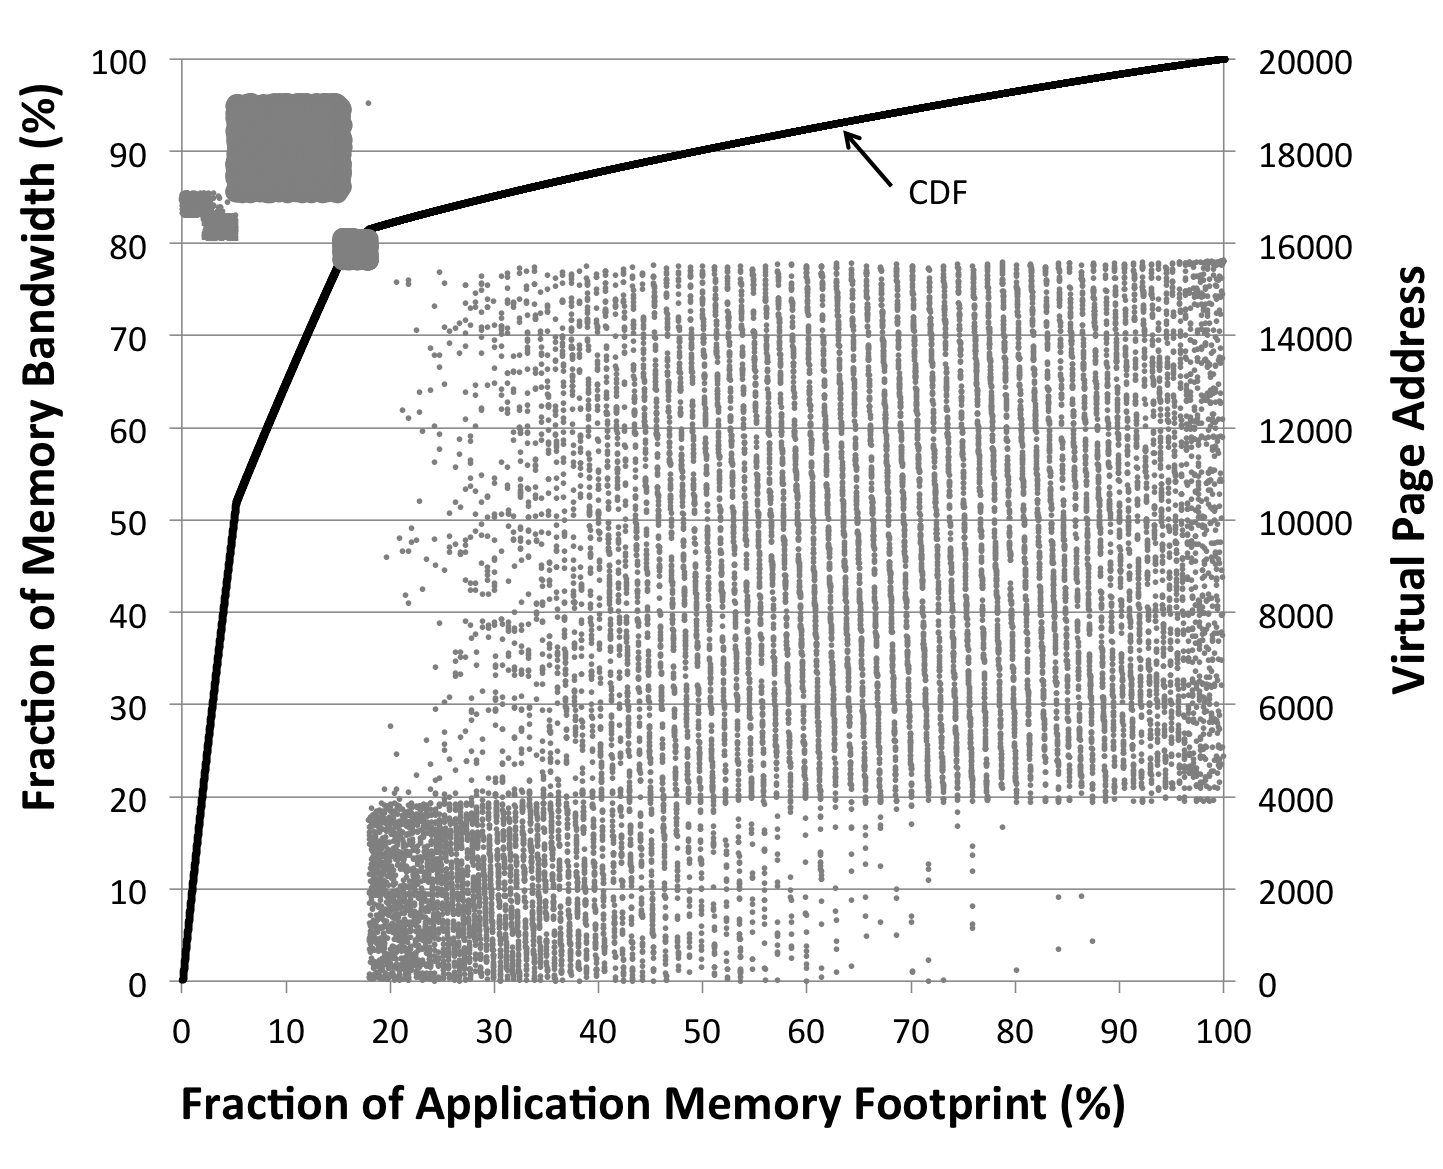
\includegraphics[width=\columnwidth]{hpca2015/figures/bfsannotated.png}}\\
    \subfloat[xsbench]{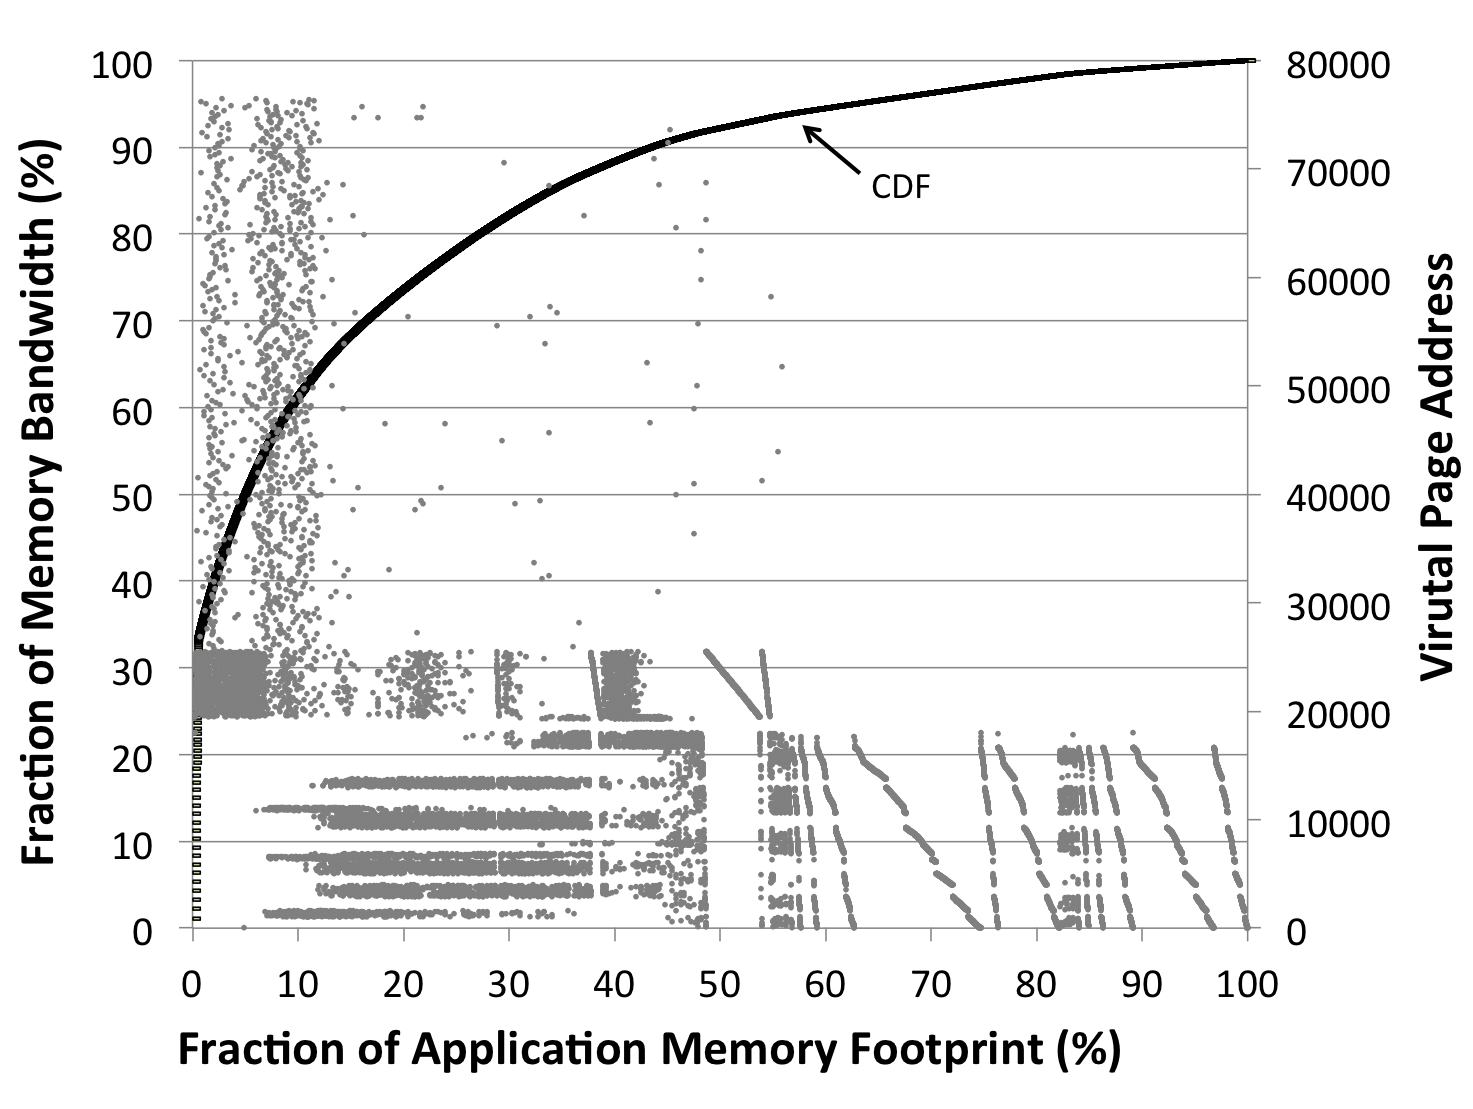
\includegraphics[width=\columnwidth]{hpca2015/figures/xsbenchannotated.png}}\\
    \subfloat[needle]{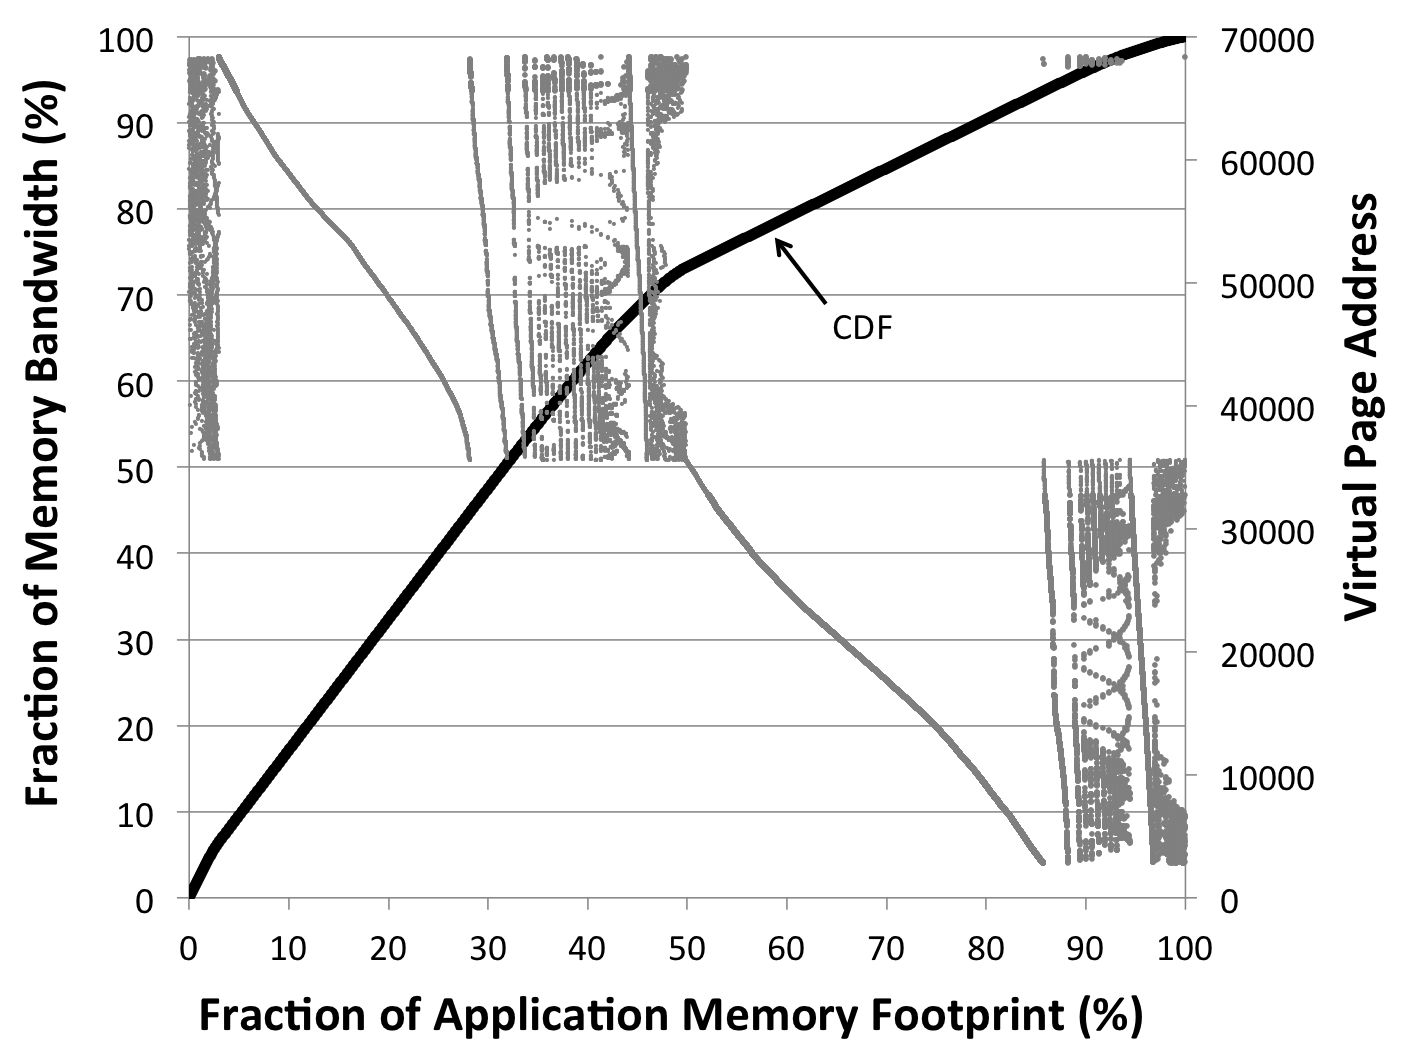
\includegraphics[width=\columnwidth]{hpca2015/figures/needleannotated.png}}\\
    \caption{Cumulative distribution of memory bandwidth versus application footprint.  Secondary axis
    shows virtual page address of pages touched when sorted by access frequency.}
    \label{fig:cdfannotation}
\end{figure}

In the case that range expansion
includes virtual addresses that are not valid, the software runtime simply allows the {\tt move\_pages}
system call to fail.  This scheme eliminates the need for additional runtime checking or data structure
overhead beyond what is already done within the operating system as part of page table tracking.
In some cases, a range expansion may extend beyond one logical data structure into another that is laid
out contiguously in the virtual address space.  While migrating these pages may be sub-optimal from a
performance standpoint, there is no correctness issue with migrating these pages to GDDR.  For
HPC-style workloads with large, coarse-grained memory allocations, this problem happens rarely in practice.

\subsection{Avoiding TLB Shootdowns With Range Expansion}
Figure~\ref{fig:migrationoverheads} shows that TLB invalidations introduce significant overheads to DDR-to-GDDR 
migrations.  Today, operating systems maintain a list of all processors that have referenced a page
so that, upon modification of the page table, TLB shootdowns are only sent to those processor cores 
(or IOMMU units in the future) that may have a cached translation for this page.  While this sharers list
may contain false positives, because the mapping entry within a particular sharer may have since been evicted from 
their TLB, it guarantees that if no request has been made for the page table entry, that core will not receive a TLB 
shootdown request.

In our previous threshold-based experiments, pages are migrated after the GPU has touched them.
This policy has the unfortunate side-effect that all page migrations will result in a TLB shootdown
on the GPU\@.  By using range expansion to identify candidates for migration that the GPU is likely to touch 
but has not yet touched, no TLB shootdown is required (as long as the page is in fact migrated before the 
first GPU touch).  As a result, range expansion provides the dual benefits of prefetching and reducing the 
number of costly TLB shootdowns.

\subsection{Results}
\label{rangeexpansionresults}
To evaluate the benefits of range expansion, we examine the effect that range expansion has when
building on our prior threshold-based migration policies.  We considered several thresholds from 1--128 accesses because, while 
the lowest threshold appears to have performed best in the absence of range expansion, it could be that using a higher
threshold, thus identifying only the hottest pages, combined with aggressive range expansion would result in improved performance. 
We model a fixed TLB shootdown overhead of 100 cycles  when performing these experiments, matching the baseline assumptions in the preceding section.

\begin{figure*}[t]
    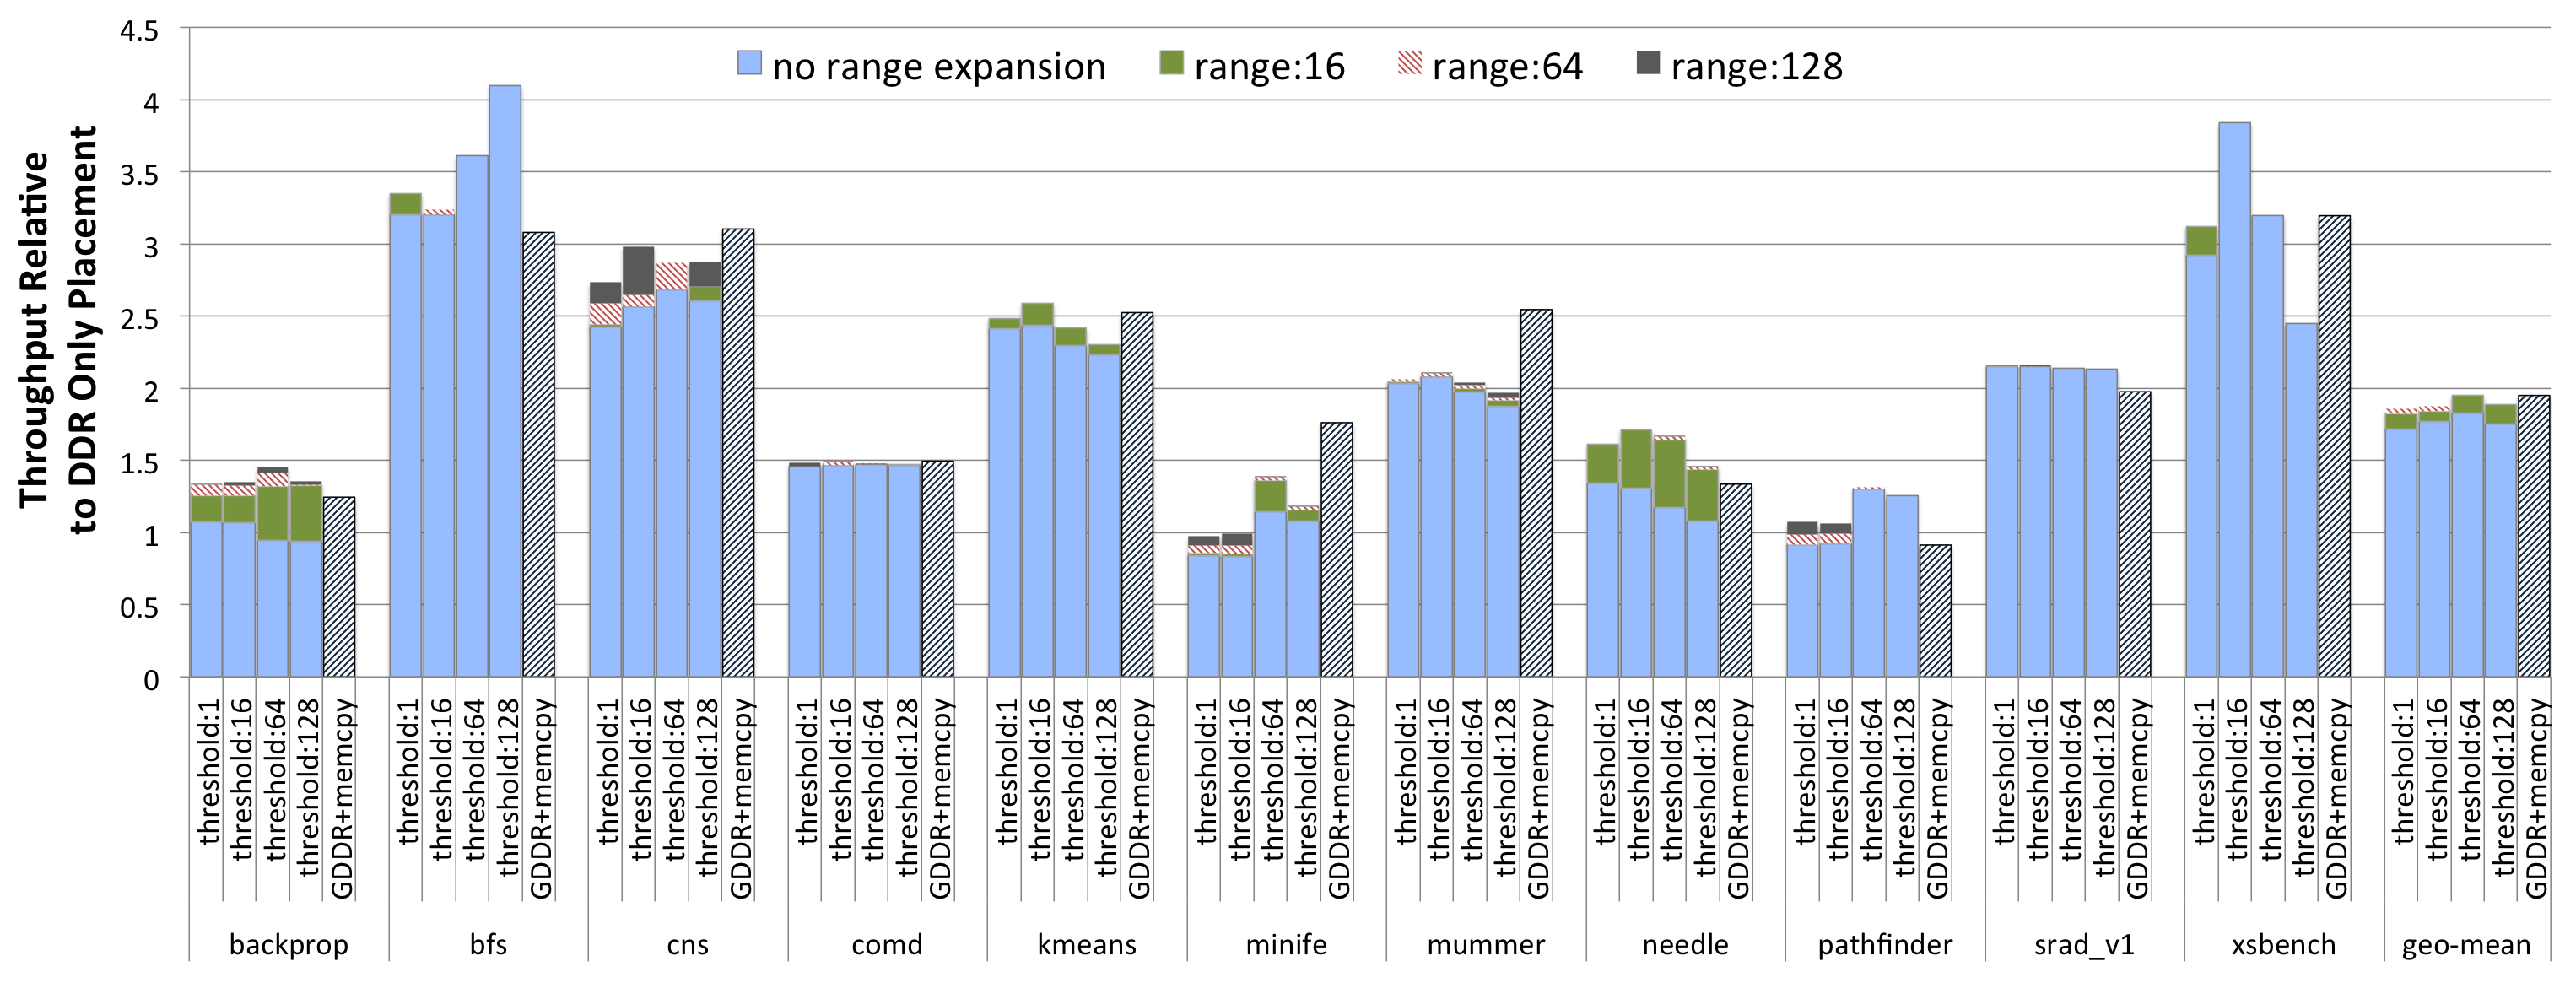
\includegraphics[width=\textwidth]{hpca2015/figures/thresh-rangeExp.png} 
    \caption{Effect of range expansion on workload performance when used in conjunction with threshold based migration.}
    \label{fig:rangeexpansion}
\end{figure*}

Figure~\ref{fig:rangeexpansion} shows application performance as a stacked bar chart on top of the
the baseline threshold-based page migration policy for various range expansion values.
For the different range expansion values, a single migration trigger is expanded to the surrounding 16, 64, or 128 
virtually addressed pages that fall within a single allocation (i.e., were
allocated in the same call to {\tt malloc}).
The pages identified via range expansion are added to the page migration list in order of furthest, 
to nearest pages from the triggered virtual address. Pages that are farther from the (already accessed) trigger
page are less likely to have been touched by the GPU yet and hence are
least likely to be cached in the GPU's TLB. These pages therefore do not
require expensive TLB shootdowns and pipeline stalls.

We see that range expansion allows us to outperform not only CC-NUMA access to DDR, but ---in many cases--- performance
exceeds that of the legacy GDDR+{\tt memcpy} implementation.  These results indicate that aggressive prefetching, 
based on first touch access information, provides a balanced method of using both DDR and GDDR
memory bandwidth.  To understand the improvement 
from the reduction in TLB shootdowns, we report the fraction of 
page migrations that required no TLB shootdown in Table~\ref{tab:shootdowns} (second column).  Compared to  
threshold-based migrations without range expansion, where all migrations incur a TLB shootdown, range expansion 
eliminates 33.5\% of TLB shootdowns on average and as many as 89\% for some applications, drastically 
reducing the performance impact of these shootdowns.

\begin{table}[bh!]
\begin{center}
\begin{small}
\begin{tabular}{|l|c|c|c|}
\hline
Benchmark & Execution & \% Migrations & Exececution\\
          & Overhead of        &Without  & Runtime\\
          & TLB Shootdowns    & Shootdown & Saved\\
\hline
backprop & 29.1\%& 26\% & 7.6\%\\
bfs & 6.7\%&12\% & 0.8\%\\
cns & 2.4\%&20\% & 0.5\%\\
comd & 2.02\%&89\% & 1.8\%\\
kmeans & 4.01\%&79\% & 3.17\%\\
minife & 3.6\%&36\% & 1.3\%\\
mummer & 21.15\%&13\% & 2.75\%\\
needle & 24.9\%&55\% & 13.7\%\\
pathfinder & 25.9\%&10\% & 2.6\%\\
srad\_v1 & 0.5\%&27\% & 0.14\%\\
xsbench & 2.1\%&1\% & 0.02\%\\
\hline
Average & 11.13\%&33.5\% & 3.72\%\\
\hline
\end{tabular}
\caption{Effectiveness of range prefetching at avoiding TLB shootdowns and runtime savings under a 100-cycle TLB shootdown overhead.}
\label{tab:shootdowns}
\end{small}
\end{center}
\end{table}

Figure~\ref{fig:rangeexpansion} shows, for {\tt bfs} and {\tt xsbench}, that range expansion provides minimal
benefit at thresholds $>$ 1. In these benchmarks, the first touches to
contiguous pages are clustered in time, because the algorithms are designed to use blocked access to the key 
data structures to enhance locality. Thus, the prefetching effect of range
expansion is only visible when a page is migrated upon first touch to a
neighboring page, by the second access to a page, all its neighbors have already been accessed 
at least once and there will be no savings from avoiding TLB shootdowns. On the other hand, in benchmarks 
such as {\tt needle}, there is low temporal correlation among touches to neighboring pages.
Even if a migration candidate is touched 64 or 128 times, some of its
neighboring pages may not have been touched, and thus the prefetching
effect of range expansion provides up to 42\% performance improvement even at higher thresholds.

In the case of {\tt backprop}, we can see that higher thresholds perform poorly
compared to threshold 1. Thresholds above 64 are simply too high; most pages are not accessed
this frequently and thus few pages are migrated, resulting in poor GDDR bandwidth utilization.
Range expansion prefetches these low-touch pages to GDDR as well, recouping the performance losses 
of the higher threshold policies and making them perform similar to a first touch migration policy.
For {\tt minife}, previously discussed in subsection~\ref{thresholdresults}, the effect of prefetching
via range expansion is to recoup some of the performance loss due to needless migrations. However,
performance still falls short of the legacy {\tt memcpy} approach, which in effect, achieves perfect prefetching.
Overuse of range expansion hurts performance in some cases. Under the 
first touch migration policy (threshold-1), using range expansion 16, 64, and 128, the worst-case
performance degradations are 2\%, 3\%, and 2.5\% respectively. While not visible in the graph due to the stacked
nature of Figure~\ref{fig:rangeexpansion}, they are included in the geometric mean calculations.

Overall, we observe that even with range expansion, higher-threshold policies
do not significantly outperform the much simpler first-touch policy. 
With threshold 1, the average performance gain with range expansion of 128 is
1.85$\times$.  The best absolute performance is observed when using a threshold of
64 combined with a range expansion value of 64, providing 1.95$\times$ speedup.
We believe that this additional $\approx$5\% speedup over first touch migration with
aggressive range expansion is not worth the implementation complexity of
tracking and differentiating all pages in the system. In the next section, we discuss how
to recoup some of this performance for benchmarks such as {\tt bfs} and {\tt xsbench}, which 
benefit most from using a higher threshold.
